%\documentstyle[epsf,twocolumn]{jarticle}       %LaTeX2e仕様
\documentclass[twocolumn]{jarticle}     %pLaTeX2e仕様(platex.exeの場合)
% \documentclass[onecolumn]{ujarticle}   %pLaTeX2e仕様(uplatex.exeの場合)
%%%%%%%%%%%%%%%%%%%%%%%%%%%%%%%%%%%%%%%%%%%%%%%%%%%%%%%%%%%%%%
%%
%%  基本バージョン
%%
%%%%%%%%%%%%%%%%%%%%%%%%%%%%%%%%%%%%%%%%%%%%%%%%%%%%%%%%%%%%%%%%
\setlength{\topmargin}{-45pt}
%\setlength{\oddsidemargin}{0cm}
\setlength{\oddsidemargin}{-7.5mm}
%\setlength{\evensidemargin}{0cm}
\setlength{\textheight}{24.1cm}
%setlength{\textheight}{25cm}
\setlength{\textwidth}{17.4cm}
%\setlength{\textwidth}{172mm}
\setlength{\columnsep}{11mm}

%\kanjiskip=.07zw plus.5pt minus.5pt


% 【節が変わるごとに (1.1)(1.2) … (2.1)(2.2) と数式番号をつけるとき】
%\makeatletter
%\renewcommand{\theequation}{%
%\thesection.\arabic{equation}} %\@addtoreset{equation}{section}
%\makeatother

%\renewcommand{\arraystretch}{0.95} 行間の設定
%%%%%%%%%%%%%%%%%%%%%%%%%%%%%%%%%%%%%%%%%%%%%%%%%%%%%%%%
%\usepackage{graphicx}   %pLaTeX2e仕様(\documentstyle ->\documentclass)
\usepackage[dvipdfmx]{graphicx}
\usepackage{subcaption}
\usepackage{multirow}
\usepackage{amsmath}
\usepackage{url}
\usepackage{ulem}
\usepackage{algorithm}
\usepackage{algorithmic}
\usepackage{listings} %,jlisting} %日本語のコメントアウトをする場合jlistingが必要
%ここからソースコードの表示に関する設定
\lstset{
  basicstyle={\ttfamily},
  identifierstyle={\small},
  commentstyle={\smallitshape},
  keywordstyle={\small\bfseries},
  ndkeywordstyle={\small},
  stringstyle={\small\ttfamily},
  frame={tb},
  breaklines=true,
  columns=[l]{fullflexible},
  numbers=left,
  xrightmargin=0zw,
  xleftmargin=3zw,
  numberstyle={\scriptsize},
  stepnumber=1,
  numbersep=1zw,
  lineskip=-0.5ex
}
%%%%%%%%%%%%%%%%%%%%%%%%%%%%%%%%%%%%%%%%%%%%%%%%%%%%%%%%
\begin{document}

	%bibtex用の設定
	%\bibliographystyle{ujarticle}

	\twocolumn[
		\noindent
		\hspace{1em}
		2020 年 9 月 18 日
		ゼミ資料
		\hfill
		B4 杉山 竜弥
		\vspace{2mm}

		\hrule
		\begin{center}
			{\Large \bf 進捗報告}
		\end{center}
		\hrule
		\vspace{9mm}
	]

	% ‚ここから 文章 Start!
\section{今週やったこと}
\begin{itemize}
	\item グラフ距離の計算
\end{itemize}

\section{問題設定}

\section{実験}
学習した結果のグラフにどの程度のばらつきがあるか調べるため, グラフの編集距離を求めた.
seed値0から9まで10回試行し, 学習して得たグラフと, ランダムノイズで得たグラフそれぞれの場合で編集距離の平均値を求めた.
編集距離の計算には, ライブラリのnetworkxを利用した. 編集距離の計算時間は全体でおよそ1時間かかった.

\begin{table}[tb]
  \begin{center}
    \caption{実験の設定}
    \begin{tabular}{|c|c|} \hline
      model & VGG11 \\ \hline
      Optim(model) & SGD(lr=0.01, momentum=0.9) \\ \hline
      Optim($\alpha$) & Adam(lr=0.005, $\beta$=(0.5, 0.999)) \\ \hline
      Loss & Cross Entropy Loss \\ \hline
      dataset & cifar10 \\ \hline
      batch size & 64 \\ \hline
      train data & 10000 + 10000 \\ \hline
      epoch & 30 \\ \hline
    \end{tabular}
    \label{tab:setting}
  \end{center}
\end{table}

\section{結果}
%
% \begin{figure}[tb]
% 	\begin{center}
% 		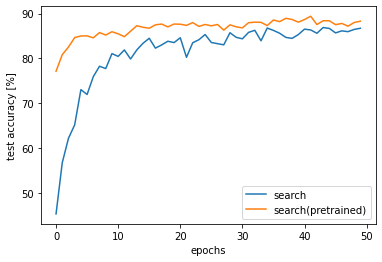
\includegraphics[clip,width=7.5cm]{acc.png}
% 		\caption{精度}
% 		\label{fig:acc}
% 	\end{center}
% \end{figure}

表\ref{tab:dist_forward}, \ref{tab:dist_random}に結果をまとめた行列を, 表\ref{tab:dist}に平均値を示した.
対称行列になるので, 下半分は計算の時間上省略した.
学習した結果, グラフにはほとんど分散はなく, ランダムの場合に比べてあるグラフに収束している.

\begin{table}[tb]
  \begin{center}
    \caption{グラフの編集距離の行列(探索した場合)}
    \begin{tabular}{|c||c|c|c|c|c|c|c|c|c|c|} \hline
      seed & 0 & 1 & 2 & 3 & 4 & 5 & 6 & 7 & 8 & 9 \\ \hline \hline
      0 & 0 & 0 & 2 & 2 & 0 & 0 & 2 & 0 & 0 & 2 \\ \hline
      1 & - & 0 & 2 & 2 & 0 & 0 & 2 & 0 & 0 & 2 \\ \hline
      2 & - & - & 0 & 4 & 2 & 2 & 2 & 2 & 2 & 2 \\ \hline
      3 & - & - & - & 0 & 2 & 2 & 4 & 2 & 2 & 4 \\ \hline
      4 & - & - & - & - & 0 & 0 & 2 & 0 & 0 & 2 \\ \hline
      5 & - & - & - & - & - & 0 & 2 & 0 & 0 & 2 \\ \hline
      6 & - & - & - & - & - & - & 0 & 2 & 2 & 2 \\ \hline
      7 & - & - & - & - & - & - & - & 0 & 0 & 2 \\ \hline
      8 & - & - & - & - & - & - & - & - & 0 & 2 \\ \hline
      9 & - & - & - & - & - & - & - & - & - & 0 \\ \hline
    \end{tabular}
    \label{tab:dist_forward}
  \end{center}
\end{table}

\begin{table}[tb]
  \begin{center}
    \caption{グラフの編集距離の行列(ランダム)}
    \begin{tabular}{|c||c|c|c|c|c|c|c|c|c|c|} \hline
      seed & 0 & 1 & 2 & 3 & 4 & 5 & 6 & 7 & 8 & 9 \\ \hline \hline
      0 & 0 & 6 & 6 & 6 & 6 & 6 & 8 & 6 & 6 & 6 \\ \hline
      1 & - & 0 & 6 & 6 & 4 & 6 & 4 & 8 & 6 & 6 \\ \hline
      2 & - & - & 0 & 6 & 6 & 4 & 6 & 4 & 6 & 6 \\ \hline
      3 & - & - & - & 0 & 6 & 6 & 6 & 4 & 6 & 4 \\ \hline
      4 & - & - & - & - & 0 & 4 & 6 & 6 & 8 & 6 \\ \hline
      5 & - & - & - & - & - & 0 & 6 & 6 & 8 & 6 \\ \hline
      6 & - & - & - & - & - & - & 0 & 6 & 2 & 4 \\ \hline
      7 & - & - & - & - & - & - & - & 0 & 6 & 4 \\ \hline
      8 & - & - & - & - & - & - & - & - & 0 & 4 \\ \hline
      9 & - & - & - & - & - & - & - & - & - & 0 \\ \hline
    \end{tabular}
    \label{tab:dist_random}
  \end{center}
\end{table}


\begin{table}[tb]
  \begin{center}
    \caption{グラフの編集距離}
    \begin{tabular}{|c||c|c|c|c|c|c|c|c|c|c|} \hline
       & mean & std \\ \hline \hline
      searched & 1.4667 & 1.1599 \\ \hline
      random & 5.6444 & 1.2276 \\ \hline
    \end{tabular}
    \label{tab:dist}
  \end{center}
\end{table}


%
% \begin{table*}[tb]
%   \begin{center}
%     \caption{$\alpha$の重み}
%     \begin{tabular}{|c|c|c|c|c|c|c|c|c|} \hline
%       i \verb|\| j & 1 & 2 & 3 & 4 & 5 & 6 \\ \hline
%       1 & 0.0000 & 0.0000 & 0.0000 & 0.0000 & 0.0000 & 0.0000 \\ \hline
%       2 & 0.0000 & 0.0000 & 0.0000 & 0.0000 & 0.0000 & 0.0000 \\ \hline
%       3 & 0.0000 & 0.0000 & 0.0000 & 0.0000 & 0.0000 & 0.0000 \\ \hline
%       4 & -0.6871 & 0.6871 & 0.0000 & 0.0000 & 0.0000 & 0.0000 \\ \hline
%       5 & -0.1982 & -0.7329 & 0.9261 & 0.0000 & 0.0000 & 0.0000 \\ \hline
%       6 & -0.6557 & 1.9855 & -0.6870 & -0.6411 & 0.0000 & 0.0000 \\ \hline
%       7 & -0.6814 & 2.4581 & -0.6656 & -0.6325 & -0.6629 & 0.0000 \\ \hline
%       8 & -0.1647 & 0.0171 & 0.3440 & 0.4793 & 0.5046 & -1.1853 \\ \hline
%     \end{tabular}
%     \label{tab:alpha}
%   \end{center}
% \end{table*}

\section{考察}

\section{今後の予定}
% なんとなくなんかの勉強をするとかではなく具体的に

% \begin{itemize}
%   \item アーキテクチャの性能評価
% \end{itemize}

\section{ソースコード}
% 埋め込みでもGitでもいいので参照できるように


% 参考文献リスト
\bibliographystyle{unsrt}
\bibliography{ref}
\end{document}
